

\tikzset{every picture/.style={line width=0.75pt}} %set default line width to 0.75pt        




\newcommand{\pointedperson}[2]{
  \node[inner sep=0.1mm] (#1#2) at (#1, #2) {\faUser};
}


\newcommand{\person}[2]{
  \node[gray, inner sep=0.1mm] (#1#2) at (#1, #2) {\faUser};
}
\newcommand{\linkpersons}[4]{
 \draw[gray] (#1#2)--(#3#4);
}

\newcommand{\examplesocialetwork}{
    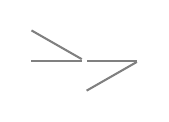
\begin{tikzpicture}[xscale=0.7, yscale=0.4]
        \pointedperson 34
        \person 14
        \person 15
        \person 24
        \person 23
        \linkpersons 3424
        \linkpersons 1524
        \linkpersons 1424
        \linkpersons 3423
    \end{tikzpicture}
}




\begin{tikzpicture}
    \node (input) at (-2.5, 0)  {\examplesocialetwork};
    \node[draw, inner sep=2mm, rounded corners=2mm] (gnn) {GNN $N$};
    \node at (2.5, 0) (output) {bot or user};
    \draw (gnn) edge[-latex] (output);
    \draw (input) edge[-latex] (gnn);
\end{tikzpicture}